\chapter{Einleitung}
\label{sec:einleitung}

Cloud Computing gehört derzeit immer noch zu einem der wichtigsten Schlagwörtern für Betreiber von IT Infrastrukturen.
\glqq Eine breit akzeptierte Definition des Begriffs Cloud Computing gibt es bis heute nicht. Allerdings können die grundlegenden Eigenschaften wie folgt zusammengefasst werden: Cloud Computing nutzt Virtualisierung und das Internet zur dynamischen Bereitstellung von IT-Ressourcen. Dabei kann es sich um IT-Infrastrukturen. Plattformen oder Anwendungen aller Art handeln. Cloudcomputing bezeichnet also sowohl Anwendungen, welche als Dienste über das Internet angeboten werden, als auch auf die Hard- und Software.\grqq \cite[S. 28]{meinel_virtualisierung_2011}

Virtualisierung und Cloud Computing sind zweit sehr stark miteinander vernetzte Begriffe.
Dabei ist Virtualisierung kein neues Konzept. Bereits in den frühen 60er Jahren entwickelte IBM mit dem Großrechnersystem 360 eine Plattform die aus heutiger Sicht als Vorläufer aller virtuellen Systeme gilt. \cite{frank_balmes_grin_????}

Heute ermöglicht uns Virtualisierung auf \glqq allen Ebenen von der Entwicklung bis zum Betrieb von Ressourcen, die Vereinheitlichung von Umgebungen und erhöhte Sicherheit durch Isolation. Dies spart Zeit bei der Entwicklung, reduziert Kosten beim Betrieb von Servern und verringert das Fehlerpotential.\grqq \cite[S. 1]{schroder_container-virtualisierung_2014}
Neben der Vollwertigen \grq Virtualisierung in Software\grq\ und der \grq Hardware-Virtualisierung\grq\ hat sich noch das Konzept der \grq Virtualisierung mittels Container\grq\ herausgebildet.
\glqq Hier wird eine komplette Betriebssystemumgebung innerhalb eines abgeschlossenen Containers zur Verfügung gestellt. Charakteristisch für diese Virtualisierungsform ist, dass nur ein Kernel des Betriebssystems läuft, der die jeweiligen Container verwaltet und eine saubere Trennung sicherstellt.\grqq \cite{plotner_linux_2012}
Seit der Kernelversion 2.6.29 \cite{fischer_linux_2014} bietet Linux eine Umsetzung dieser Virtualisierungsform bereits als festen Bestandteil des Betriebssystems.
Das Problem mit diesen als \grq LXC\grq\ bekannten Containern ist jedoch ihre sehr unhandliches Interface.
Das Open Source Projekt \grq Docker\grq\ der Firma \grq dotCloud\grq\ hat sich diesem Problem angenommen und eine benutzerfreundliche Abstraktionsschicht für die Verwendung von LXC Containern entwickelt. Das Projekt steckt zwar immer noch in den Kinderschuhen, erfreut sich aber schnell wachsender Beliebtheit, wie der Trend der Suchanfragen nach dem Begriff \grq Docker\grq\ anzeigt.

\begin{figure}[htb]
  \centering  
  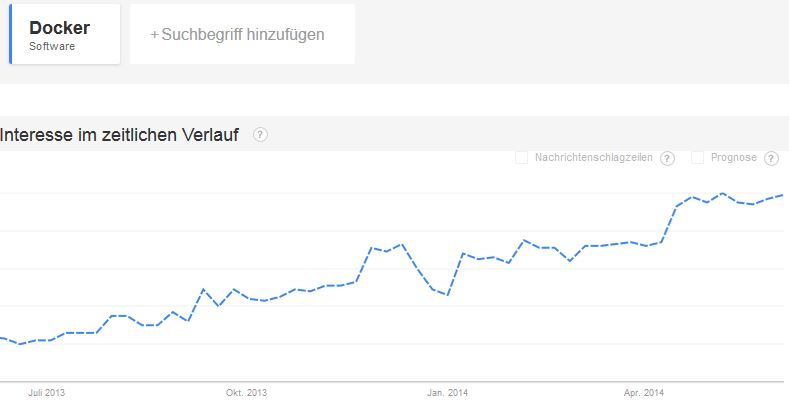
\includegraphics[scale=0.7]{img/docker_trend.JPG}\\
  \footnotesize\sffamily\textbf{Quelle:} \cite{google_trends_google_2014}
  \caption{Trend der Suchanfragen nach dem Begriff \grq Docker\grq\ im Bereich von 07.06.2013 - 07.06.2014 }
  \label{fig:iaas_paas_saas}
\end{figure}

Bereits innerhalb der ersten acht Monaten seit dem Start des Projekts wuchs die Zahl der beitragenden Personen auf über zweihundert an. 
Heute ist Docker bereits in namenhaften Projekten wie \grq Jenkins\grq\, \grq Travis\grq\ oder \grq Vagrant\grq\ integriert. \cite{hykes_docker_2013}
Da Docker auf LXC basiert hat es den großen Vorteil auf allen aktuellen Linuxsystemen ohne Änderungen zu laufen. Es erweitert LXC um eine benutzerfreundliche Schnittstelle zum erzeugen, verwalten und persistieren von Containern und übernimmt die Konfigurationder der Inter-Container-
Kommunikation. Das ursprüngliche Ziel das Docker dabei verfolgt ist es Anwendungen mittels Containern in einen zuvor definierten, immer gleichen Kontext zu stellen. Die so in einen Container eingebetteten Anwendungen sollen dann unabhängig von der vorherrschenden Systemkonfiguration auf jedem beliebigen Hostsystem ausführbar sein.
Zum verwalten der Container setzt Docker auf ein Versionskontrollsystem ähnlichen Ansatz.
Neue Container werden immer ausgehend von einem bereits existierendem Stand gebildet und gespeichert. Änderungen an Containern werden damit sehr klein und sind dadurch besonders effizient zu übertragen.
Durch die Vereinfachung der Verwendung von LXC Containern öffnet Docker die Türe zu eine Vielzahl von möglichen Anwendungsszenarien die vor allem den Bereich des Cloudcomputing vereinfachen und unterstützen können.
Die Folgende Arbeit betrachtet eine Auswahl dieser Anwendungsszenarien.